\documentclass[answers]{exam}

%% Language and font encodings
\usepackage[english]{babel}
\usepackage[utf8x]{inputenc}
\usepackage[T1]{fontenc}
% \usepackage{enumitem}
%% Sets page size and margins
\usepackage[a4paper,margin=2cm]{geometry}

%% Useful packages
\usepackage{amsmath}
\usepackage{amssymb}
\usepackage{graphicx}
\usepackage{paralist}
\usepackage{framed}
\usepackage{tikz}
\usepackage{float}
\usepackage{listings}
\usepackage{xcolor}
\usepackage{subfigure}
\tikzset{
  % define the bar graph element
  bar/.pic={
    \fill (-.1,0) rectangle (.1,#1) (0,#1) node[above,scale=1/2]{$#1$};
  }
}
\definecolor{codegreen}{rgb}{0,0.6,0}
\definecolor{codegray}{rgb}{0.5,0.5,0.5}
\definecolor{codepurple}{rgb}{0.58,0,0.82}
\definecolor{backcolour}{rgb}{0.95,0.95,0.92}
% Colored Python listing from https://www.overleaf.com/learn/latex/Code_listing
\definecolor{codegreen}{rgb}{0,0.6,0}
\definecolor{codegray}{rgb}{0.5,0.5,0.5}
\definecolor{codepurple}{rgb}{0.58,0,0.82}
\definecolor{backcolour}{rgb}{0.95,0.95,0.92}
 
\lstdefinestyle{mystyle}{
    backgroundcolor=\color{backcolour},   
    commentstyle=\color{codegreen},
    keywordstyle=\color{magenta},
    numberstyle=\tiny\color{codegray},
    stringstyle=\color{codepurple},
    basicstyle=\ttfamily\footnotesize,
    breakatwhitespace=false,         
    breaklines=true,                 
    captionpos=b,                    
    keepspaces=true,                 
    numbers=left,                    
    numbersep=5pt,                  
    showspaces=false,                
    showstringspaces=false,
    showtabs=false,                  
    tabsize=2
}
\lstset{style=mystyle}

\usetikzlibrary{matrix}

\setlength\FrameSep{4pt}
\title{Probability \& Statistics\\ Project}
\author{Hana Ali Rashid, hr05940\\ Tasmiya Malik, Student ID\\ Ifrah Ilyas, Student ID}
\date{\today{}}
\begin{document}
\maketitle

% \noindent \hrulefill \\
% \textbf{Instructions:}
% \begin{itemize}
%     \item \textbf{Pairs can not be cross-section.}
% \end{itemize}

% \noindent \hrulefill

\section*{Q1: Random Walk}
\subsection*{1.1}
Function implementation in Python:
\lstinputlisting[firstline=5,lastline=13,language=python]{q1.py}
Calling the function for several iterations to get multiple expected values:
\lstinputlisting[firstline=16,lastline=31,language=python]{q1.py}
\pagebreak

\begin{figure}
  \centering
  \mbox{\subfigure[No. of steps taken = 10 with probability of moving a step right = 0.5.]{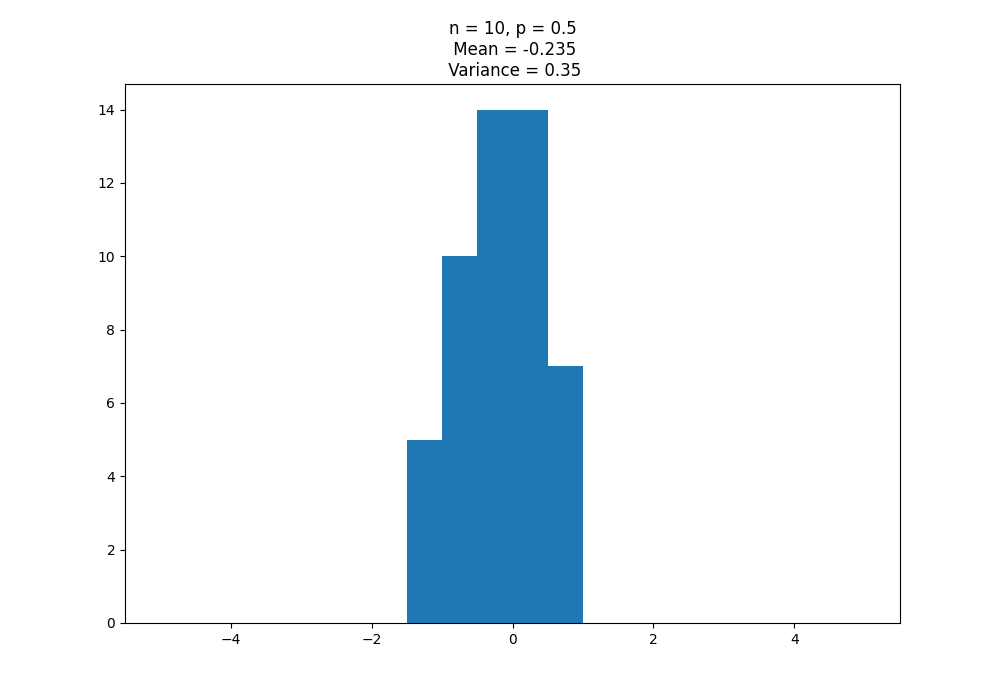
\includegraphics[scale = 0.35]{Q1_histograms/1.1/q1_n = 10_ p = 0.5.png}}\quad
  \subfigure[No. of steps taken = 18 with probability of moving a step right = 0.5.]{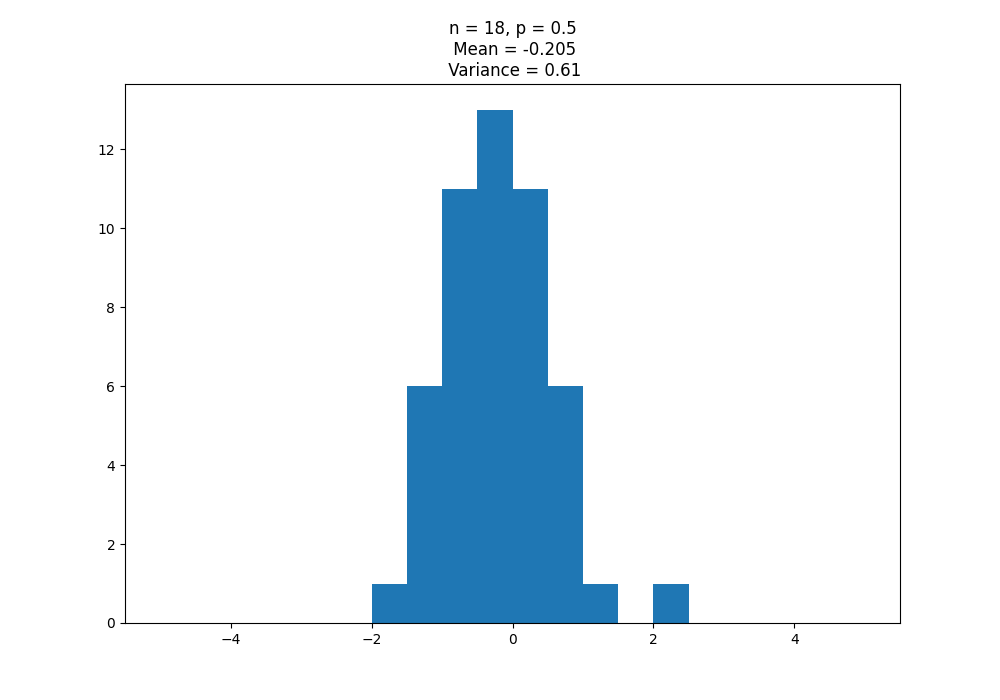
\includegraphics[scale = 0.35]{Q1_histograms/1.1/q1_n = 18_ p = 0.5.png} }}
\end{figure}
\begin{figure}
  \centering
  \mbox{\subfigure[No. of steps taken = 10 with probability of moving a step right = 0.7.]{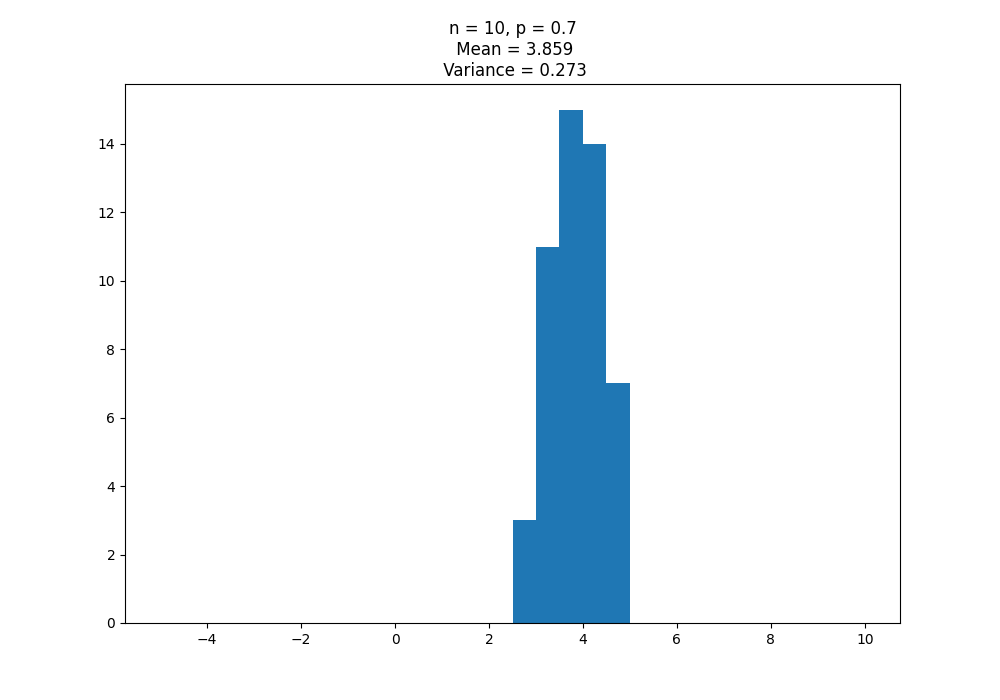
\includegraphics[scale = 0.4]{Q1_histograms/1.1/q1_n = 10_ p = 0.7.png}}}
\end{figure}

Histograms produced by the above code for expected final positions of objects against frequency, where $n$ is the number of steps taken and $p$ is the probability of the object moving one step to the right.\\
\\
Histograms $(a)$ and $(b)$ have the same value of $p$ and varying number of steps $n$. \\
Both histograms appear to follow a normal distribution, with $(a)$ having a mean of $-0.235$ and a variance of $0.35$ and $(b)$ having a mean of $-0.205$ and a variance of $0.61$. Increasing the number of steps has not had a significant effect on the mean but did increase the variance.\\ \\
Histograms $(a)$ and $(c)$ have the same number of steps $n$ and varying values of $p$. \\
Histogram $(c)$ also appears to follow a normal distribution, having a mean of $3.859$ and a variance of $0.273$. Increasing $p$ appears to have affected the mean of the distribution but not the variance as such.\\


\pagebreak
%--------------------------------  1.2  ------------------------------------
\subsection*{1.2}
Function implementation in Python:
\lstinputlisting[firstline=34,lastline=42,language=python]{q1.py}
Calling the function for several iterations to get multiple expected values:
\lstinputlisting[firstline=44,lastline=59,language=python]{q1.py}
\pagebreak

\begin{figure}
  \centering
  \mbox{\subfigure[No. of steps taken = 20 with probability of moving a step right = 0.5.]{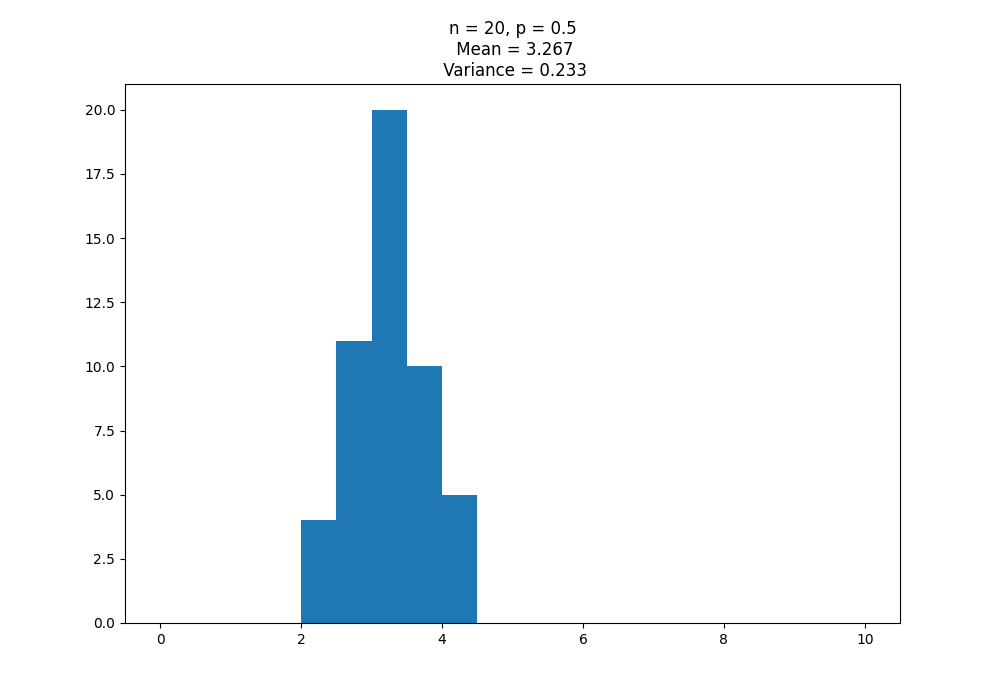
\includegraphics[scale = 0.35]{Q1_histograms/1.2/Q1.2 _n = 20_p = 0.5.png}}\quad
  \subfigure[No. of steps taken = 24 with probability of moving a step right = 0.5.]{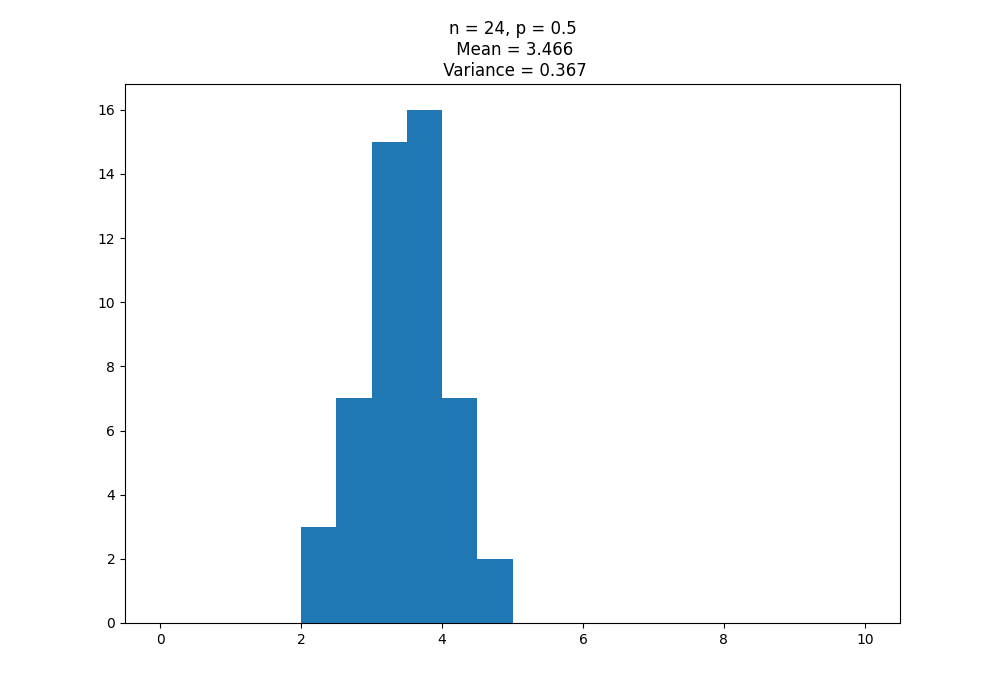
\includegraphics[scale = 0.35]{Q1_histograms/1.2/Q1.2 _n = 24_p = 0.5.png}}}
\end{figure}
\begin{figure}
  \centering
  \mbox{\subfigure[No. of steps taken = 20 with probability of moving a step right = 0.7.]{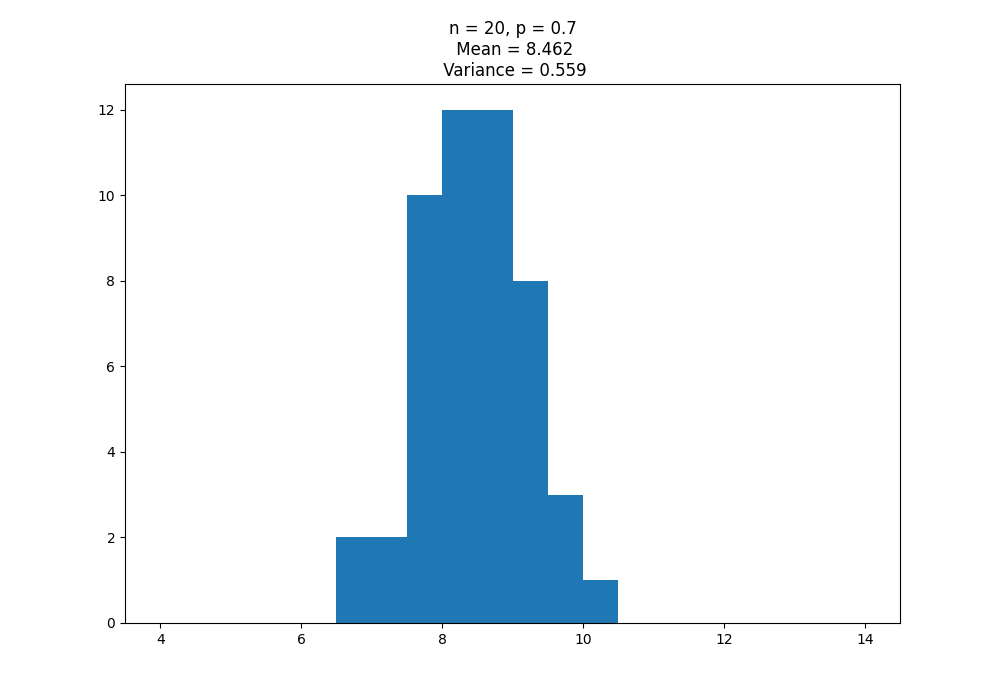
\includegraphics[scale = 0.35]{Q1_histograms/1.2/Q1.2 _n = 20_p = 0.7.png}}\quad
  \subfigure[No. of steps taken = 24 with probability of moving a step right = 0.7.]{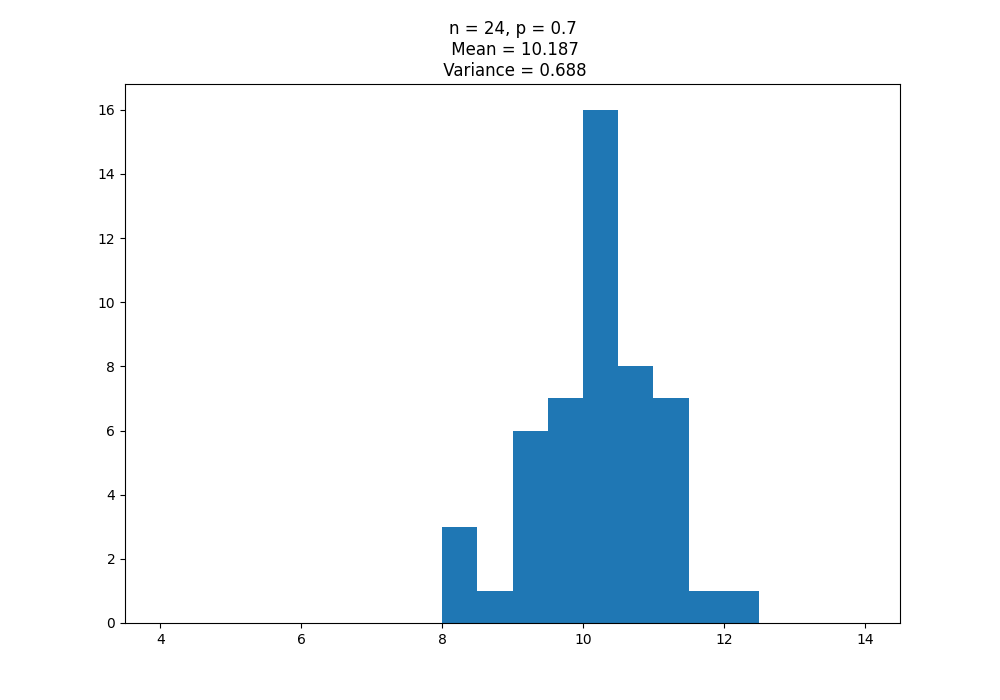
\includegraphics[scale = 0.35]{Q1_histograms/1.2/Q1.2 _n = 24_p = 0.7.png}}}
\end{figure}

Histograms produced by the above code for expected final positions of objects against frequency, where $n$ is the number of steps taken and $p$ is the probability of the object moving one step to the right.\\
\\
Histograms $(d)$ and $(e)$ have the same value of $p$ and varying number of steps $n$. \\
Both histograms appear to follow a normal distribution, with $(d)$ having a mean of $3.267$ and a variance of $0.233$ and $(e)$ having a mean of $3.466$ and a variance of $0.367$. Again, increasing the number of steps has not had a significant effect on the mean but did increase the variance.\\ \\
Histograms $(f)$ and $(g)$ have the same number of steps $n$ respectively as $(d)$ and $(e)$ and varying values of $p$. 
They also appear to follow a normal distribution, with $(f)$ having a mean of $8.462$ and a variance of $0.559$ and $(g)$ having a mean of $10.187$ and a variance of $0.668$. Increasing $p$ appears to have increased the mean and variance, but the mean has increased more significantly. \\ \\
Additionally, due to the added constraint in this part, we see that no expected value for the final position is negative.

\pagebreak
%--------------------------------  1.3  ------------------------------------
\subsection*{1.3}
Function implementation in Python:
\lstinputlisting[firstline=61,lastline=75,language=python]{q1.py}
Calling the function for several iterations to get multiple expected values:
\lstinputlisting[firstline=77,lastline=97,language=python]{q1.py}
\pagebreak
Histograms produced by the above code for expected number of steps taken for two objects walking randomly to meet, against frequency. $p1$ and $p2$ are the respective probabilities of object 1 and object 2 moving one step to the right, and $pos1$ and $pos2$ denote the starting positions of object 1 and object 2 respectively.\\

\begin{center}
  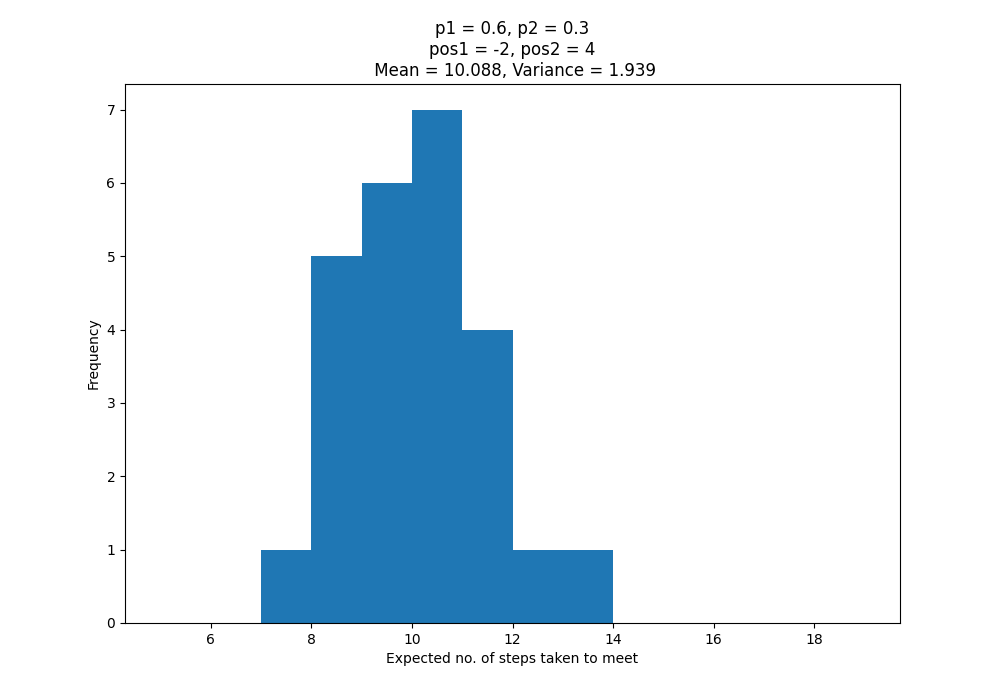
\includegraphics[scale = 0.5]{Q1_histograms/1.3/Q1.3 _p1 = 0.6_p2 = 0.3_pos1 = -2_pos2 = 4.png}
\end{center}

The above histogram shows that the expected number of steps to meet for two objects follows a normal distribution of mean $10.09$ and variance $1.94$ when they begin 6 steps apart with the given probabilities. \\
\begin{center}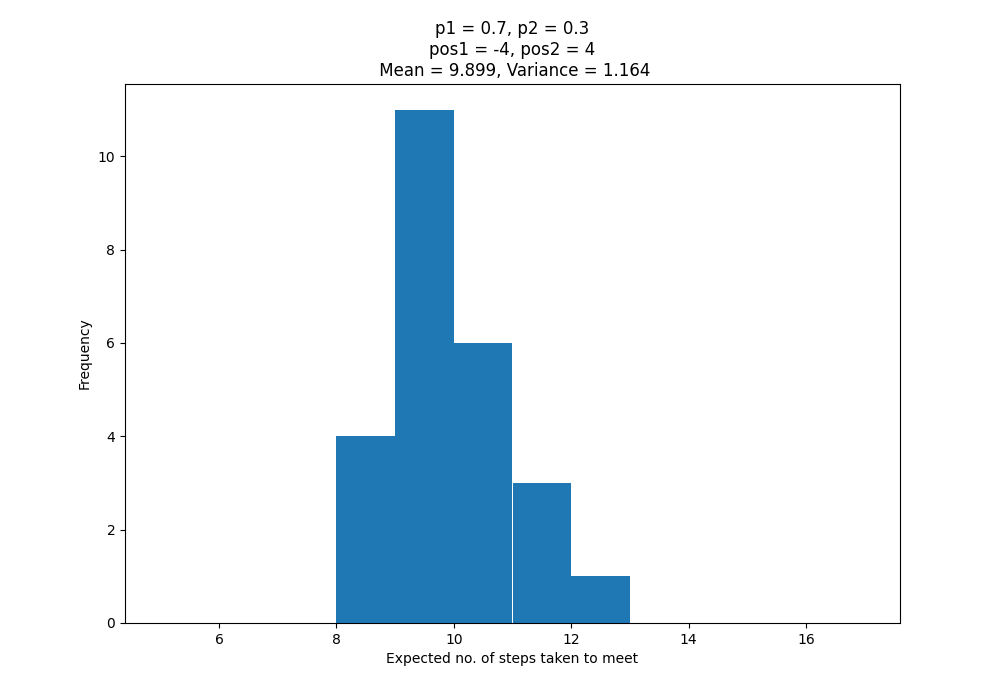
\includegraphics[scale = 0.5]{Q1_histograms/1.3/Q1.3 _p1 = 0.7_p2 = 0.3_pos1 = -4_pos2 = 4.png}\end{center}
The above histogram shows that the expected number of steps to meet for two objects follows a normal distribution of mean $9.90$ and variance $1.16$ when they begin 8 steps apart with the given probabilities. \\

% ------------------------------------------------- 5 -------------------------------------------------------------------
\pagebreak
\section*{Q5: Hypothesis Testing}
\subsection*{5.1}
Function that implements the simulation of a fair coin:
\lstinputlisting[firstline=10,lastline=12,language=python]{q5.py}
Function that uses the above function to simulate 10 coin tosses multiple times and finds the expected number of times the null hypothesis is rejected:
\lstinputlisting[firstline=14,lastline=35, language=python]{q5.py}
Histogram of expected values:
\begin{center}
  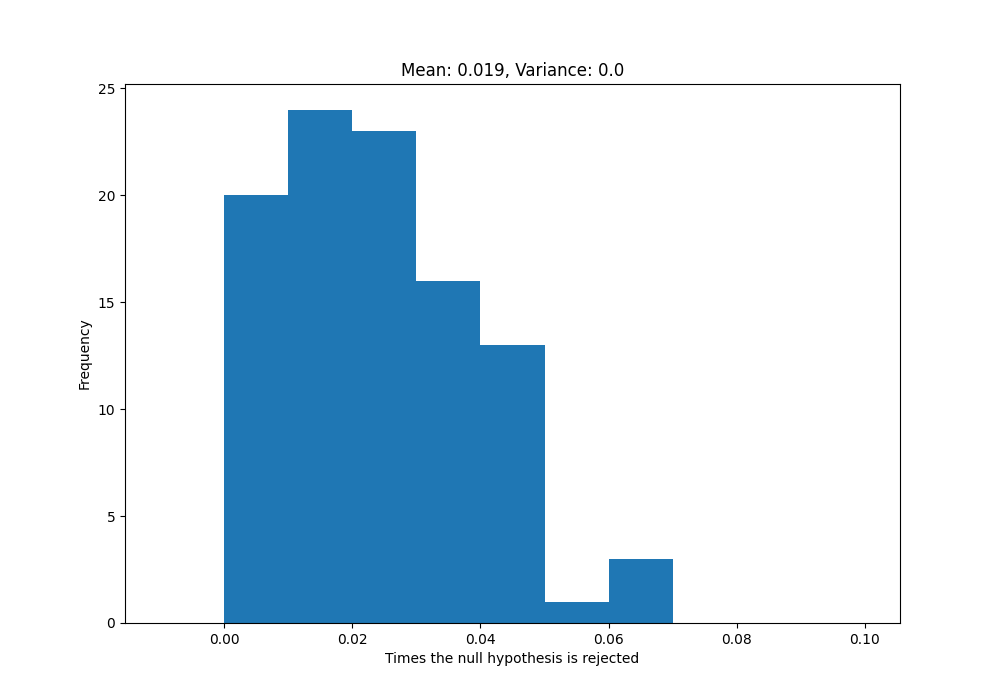
\includegraphics[scale = 0.5]{Q5_histograms/Q5.1.png}
\end{center}
Probability we will reject the null hypothesis even though it is true:\\
\emph{Simulation-wise}: According to the mean of the expected values, the probability is $2.3\%$.\\
\emph{Mathematically}: We reject the null hypothesis if the probability of the outcomes is below the threshold. Since the probability of the outcomes being accepted is 0.95 and the probability of them being rejected is 0.05, the probability that we reject the null hypothesis even though it is true is also 0.05 which is equal to the threshold.

\end{document} 